\section*{Reviewer 2}

\begin{enumerate}
	\item The additive and multiplicative effects (AME) model presented in the paper allows for a better treatment of first, second and third order dependencies in the data, and account for unobserved sources of bias in the data. The presentation of the AME estimator is clear, and the simulations provide clear evidence that the model outperforms naive OLS/GLM models fitted to the same data. The paper will be of great interest to the PSRM audience and is likely to have a strong impact on future research in international relations. I do, however, have a few suggestions for revisions that will hopefully strengthen the paper’s contributions.
	\begin{itemize}
		\item \textcolor{blue}{ \emph{
		We thank the reviewer for their comments and suggestions.
		}}
	\end{itemize}
	\item The paper shows that the AME model performs well in comparison to the “oracle” model where all sources of dependencies in the data are accounted for, which is reassuring. Yet this comparison feels incomplete. First, the naive model is clearly misspecified given the underlying data generating process. A large number of dependencies in international relations are linked to geography. What would happen if the dependencies were modeled using spatial econometric techniques?
	\begin{itemize}
		\item \textcolor{blue}{ \emph{
			The reviewer raises an important connection to the spatial literature. The types of geographic dependencies in international relations are generally monadic in nature -- civil war spreads from Rwanda to Uganda, or protest from Lebanon to Syria. With dyadic data, however, we cannot use the common geographic adjacency matrices used for normal spatial econometrics, because in dyadic data a W matrix would need to specify how dyad i,j relates to dyad k,l (for every i,j,k,l). In the simulation, we do not include a spatial lag model because this would require specifying a spatial dependence pattern (see Plumper and Neumayer 2010 for a more in-depth discuss on spatial lags). \textbf{CD}: I added this as a footnote on p.9. I moved this footnote around a LOT but I think it needs to live somewhere in the simulation. It felt awkward within the text.
			}}
%		CDMG: Flag for discussion. We brainstormed how to fit this into the simulation, but wouldn't simulating a W matrix be a bit arbitrary here?
%		Reference papers that have thought about what happens when we get the wrong W
%		general gist .. spatial models of dyadic dvs are great if we know how to characterize the diffusion amtrices, but the point of our approach is that we may not know how to actually characterize the ways in which actors are related to one another on some diffusion space.
%		reference franzesse et al mstar framework as a way to operationalize multiple pathways of diffusion in a spatial econometric approach
	\end{itemize}
	\item It would help if the author discussed in more depth the properties of the AME estimator in the presence of unobserved dependencies. One would imagine that the oracle model, where all the unobserved factors and dependencies are accounted for should always outperform a parametric or semi-parametric estimator. Relatedly, it also would help to have a more technical discussion of the properties of AME models, particularly in terms of the bias-variance trade off.
	\begin{itemize}
		\item \textcolor{blue}{ \emph{
		add example of case where omitted variable is correlated
		tech discussion bias-variance

		\begin{figure}[ht]
		\caption{Regression parameter estimates for the standard, AME, and oracle models from 1,000 simulations. Summary statistics are presented through a traditional box plot, and the estimates from each simulation are visualized as well as points.}
		\label{fig:ameBias}
		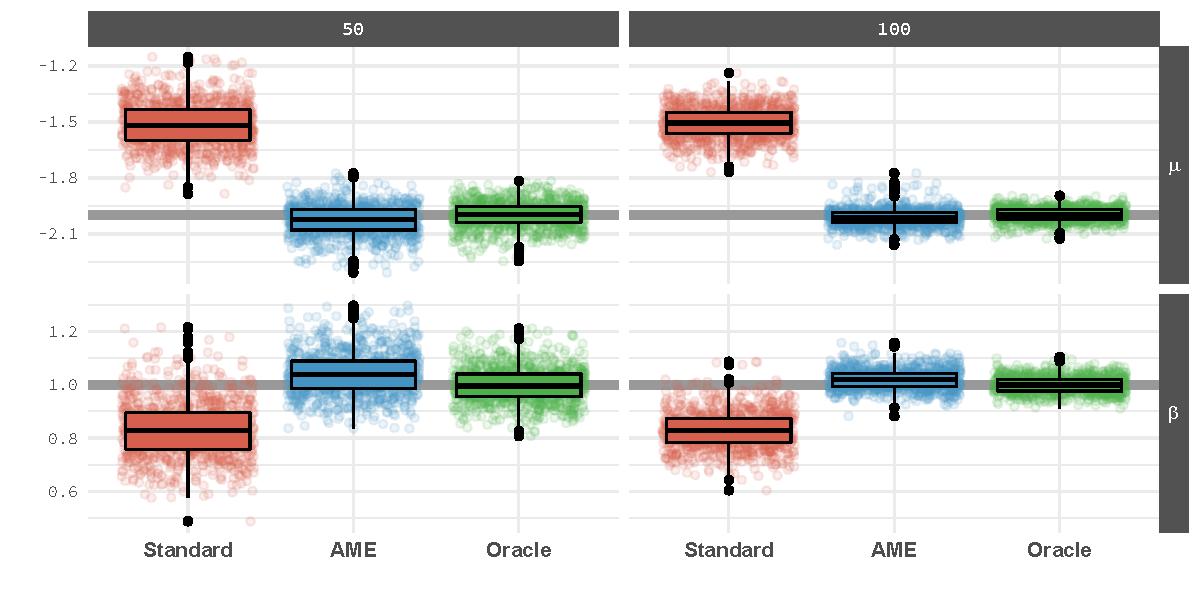
\includegraphics[width=1\textwidth]{ameSimBias_all_corrProbitMed.pdf} \\
		\end{figure}

		\begin{figure}[ht]
		\caption{Regression parameter estimates for the standard, AME, and oracle models from 1,000 simulations. Summary statistics are presented through a traditional box plot, and the estimates from each simulation are visualized as well as points.}
		\label{fig:ameBias}
		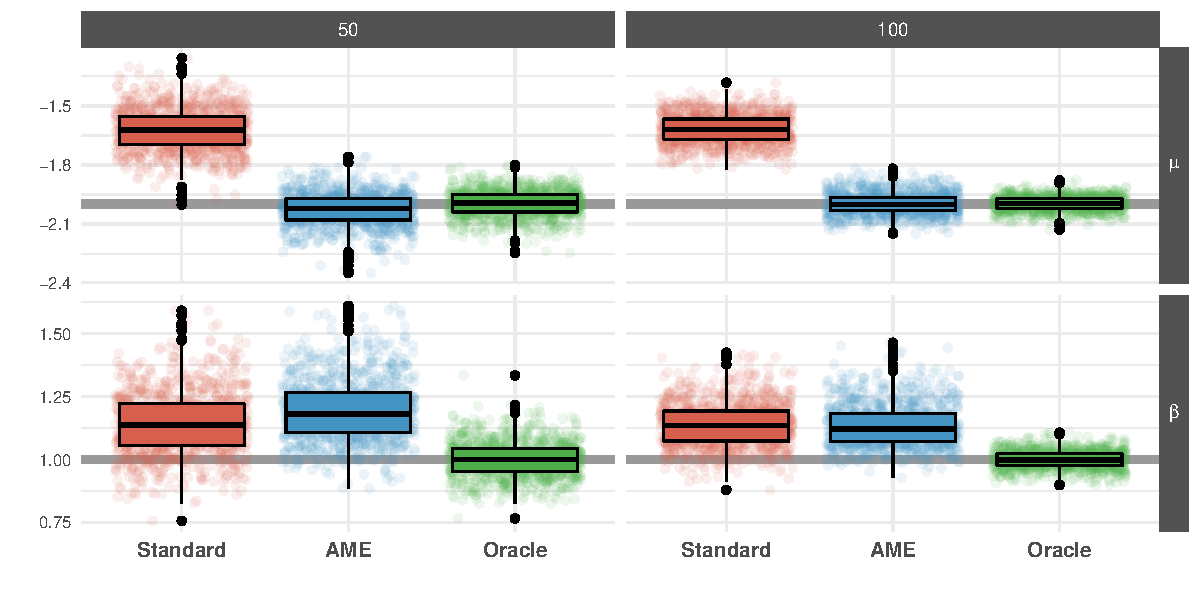
\includegraphics[width=1\textwidth]{ameSimBias_all_corrProbitHi.pdf} \\
		\end{figure}

		\begin{figure}[ht]
		\caption{Regression parameter estimates for the standard, AME, and oracle models from 1,000 simulations. Summary statistics are presented through a traditional box plot, and the estimates from each simulation are visualized as well as points.}
		\label{fig:ameBias}
		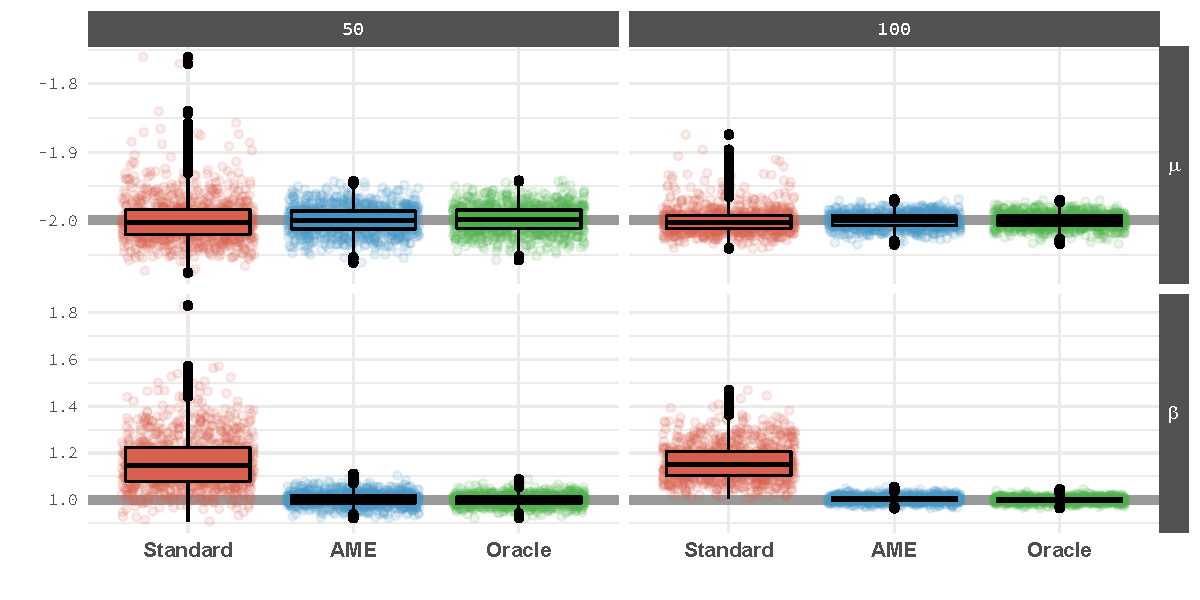
\includegraphics[width=1\textwidth]{ameSimBias_all_corrMed.pdf} \\
		\end{figure}

		\begin{figure}[ht]
		\caption{Regression parameter estimates for the standard, AME, and oracle models from 1,000 simulations. Summary statistics are presented through a traditional box plot, and the estimates from each simulation are visualized as well as points.}
		\label{fig:ameBias}
		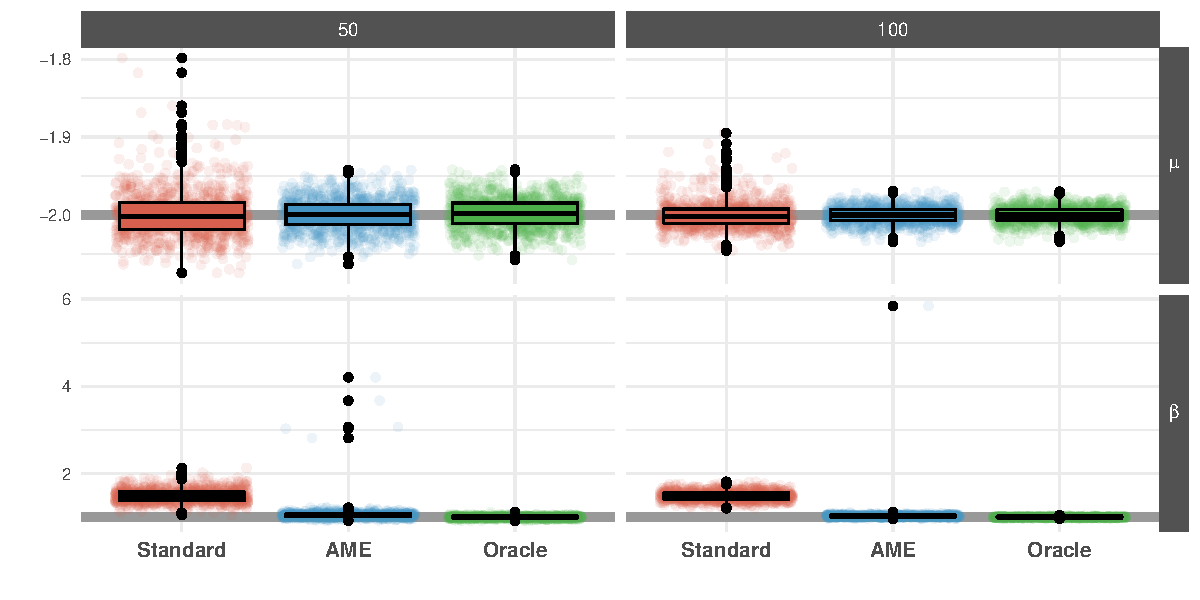
\includegraphics[width=1\textwidth]{ameSimBias_all_corrHi.pdf} \\
		\end{figure}		
		}}
	\end{itemize}
	\item The author could also underscore a related issue, which usually escapes empirical IR scholars: the importance of developing theories that account for the direct and indirect effects of interactions in a setting where the units are interconnected, and where the effects on one unit have the potential to impact other units in the system. A traditional approach is to throw as many observable variables as possible as controls, without much consideration on where they fit in the model. As the comparison of the AME and oracle models suggests, a careful modeling of spillovers and dependencies can result in better estimates of the underlying relationships.
	\begin{itemize}
		\item \textcolor{blue}{ \emph{
		We agree with this suggestion. We have now emphasized the importance of developing theory in our discussion of the AME and Oracle comparison (p. 13), as well as in the conclusion of our paper. We agree that innovations in dependence modeling can and should speak to theoretical advancements that, like our model, take into account the important relational and interdependent nature of political processes.
		}}
	\end{itemize}
	\item The paper emphasizes the importance of estimating the random effects for theory building and hypothesis test. A longer elaboration and illustration of this point would be very helpful.
	\begin{itemize}
		\item \textcolor{blue}{ \emph{
		We have added an additional interpretation of the random effects on pg. 19 in our discussion of Reiter and Stam. (``Specifically, we can see that countries such as Iraq, Israel, Egypt, and Iran are more likely to be involved in initiating or continuing conflict with other countries than the model would predict. Further, other countries such as Bhutan, Finland, and Turkmenistan are less likely to engage in conflict than the exogenous covariates in the model would suggest. In this case, the finding that countries in the middle east experience more conflict with other countries might lead one to more carefully examine the effects of geography on conflict initiation or to account for \citet{colgan:2010}'s theory that revolutionary petrostates are more aggressive.")
				}}
	\end{itemize}
	\item I would like to see a more detailed discussion of the setup and choices made for the Monte Carlo simulations. What type of network do the simulated data model? How does the network in the simulation relate to typical networks in IR studies, and to the ones in the replicated papers.
	\begin{itemize}
		\item \textcolor{blue}{ \emph{
		We've added additional discussion about how each of the variables in our simulation were generated. To make the model more applicable to the types of networks we study in IR we have provided a probit example.
		}}
	\end{itemize}
	\item The criteria for choosing the studies for replication is unclear and needs a better justification. I would have liked to see a larger set of replications particularly in areas and topics where the data generating process, the dependencies among units varies, or the relationship between the units is hierarchical, cross-classified or multilevel.
	\begin{itemize}
		\item \textcolor{blue}{ \emph{
		We selected our cases based on a few criteria. We focus on studies that are explicitly about International Relations, were published since the year 2000, and were published in a top ranking general political science outlet (for consistency in editorial standards and reviews, we also decided to focus on one journal, the APSR). We hope that these three criteria ensure that our paper is readable and interpretable to an applied audience. In addition, we selected studies that could help illustrate different key components of the AME approach such as random effects (Reiter and Stam 2003), third-order dependencies (Weeks 2012), precision of fixed effects estimates (Gibler 2017).  While we agree with the reviewer that further replications would effectively demonstrate the benefits of the AME, we believe that they are beyond the scope of this paper at this time.
		}}
	\end{itemize}
	\item Given the importance of promoting the use of the AME method I would encourage the author to revise the tutorial presented in Appendix C to make it more accessible to a larger audience.
	\begin{itemize}
		\item \textcolor{blue}{ \emph{
		The reviewer raises a valid point. We have expanded our tutorial in Appendix C, particularly in giving more detail and concrete examples when it comes to formatting the data, which may represent the biggest hurdle for some users. We also...
		}}
	\end{itemize}
\end{enumerate}
